\documentclass[../main.tex]{subfiles}
%!TEX root = ./appendixThrusterShaftAssemblySelection.tex
\graphicspath {{../}}

\begin{document}
\subsection{Motor and Propeller Selection} \label{motorSelect}

\begin{figure}[H]
	\centering
	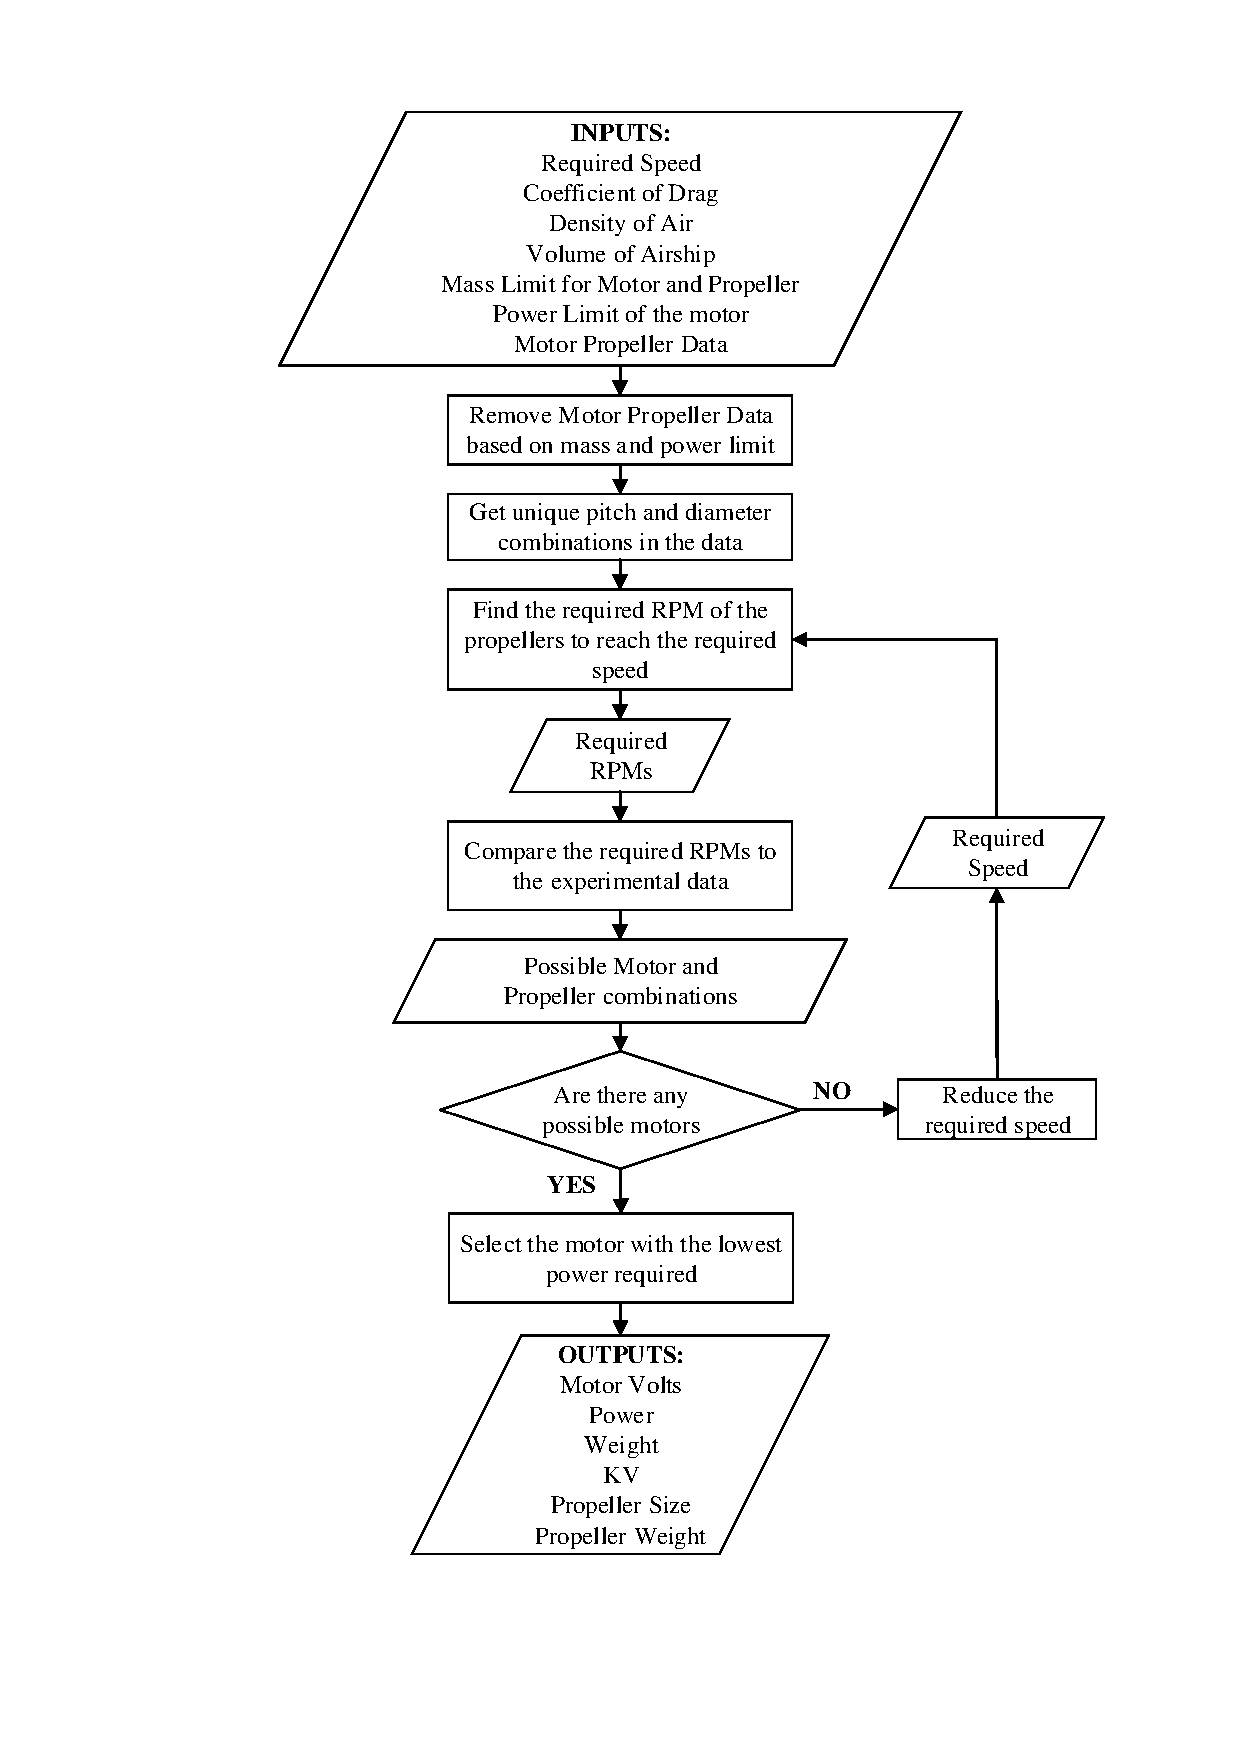
\includegraphics[width=0.7\linewidth]{img/paramaterization/motorPropellerChoice.pdf}
	\caption{Parametrization Outline For Motor and Propeller Selection}
	\label{fig:motorOutline}
\end{figure}

\subsection{Battery Selection} \label{batterySelect}

\begin{figure}[H]
	\centering
	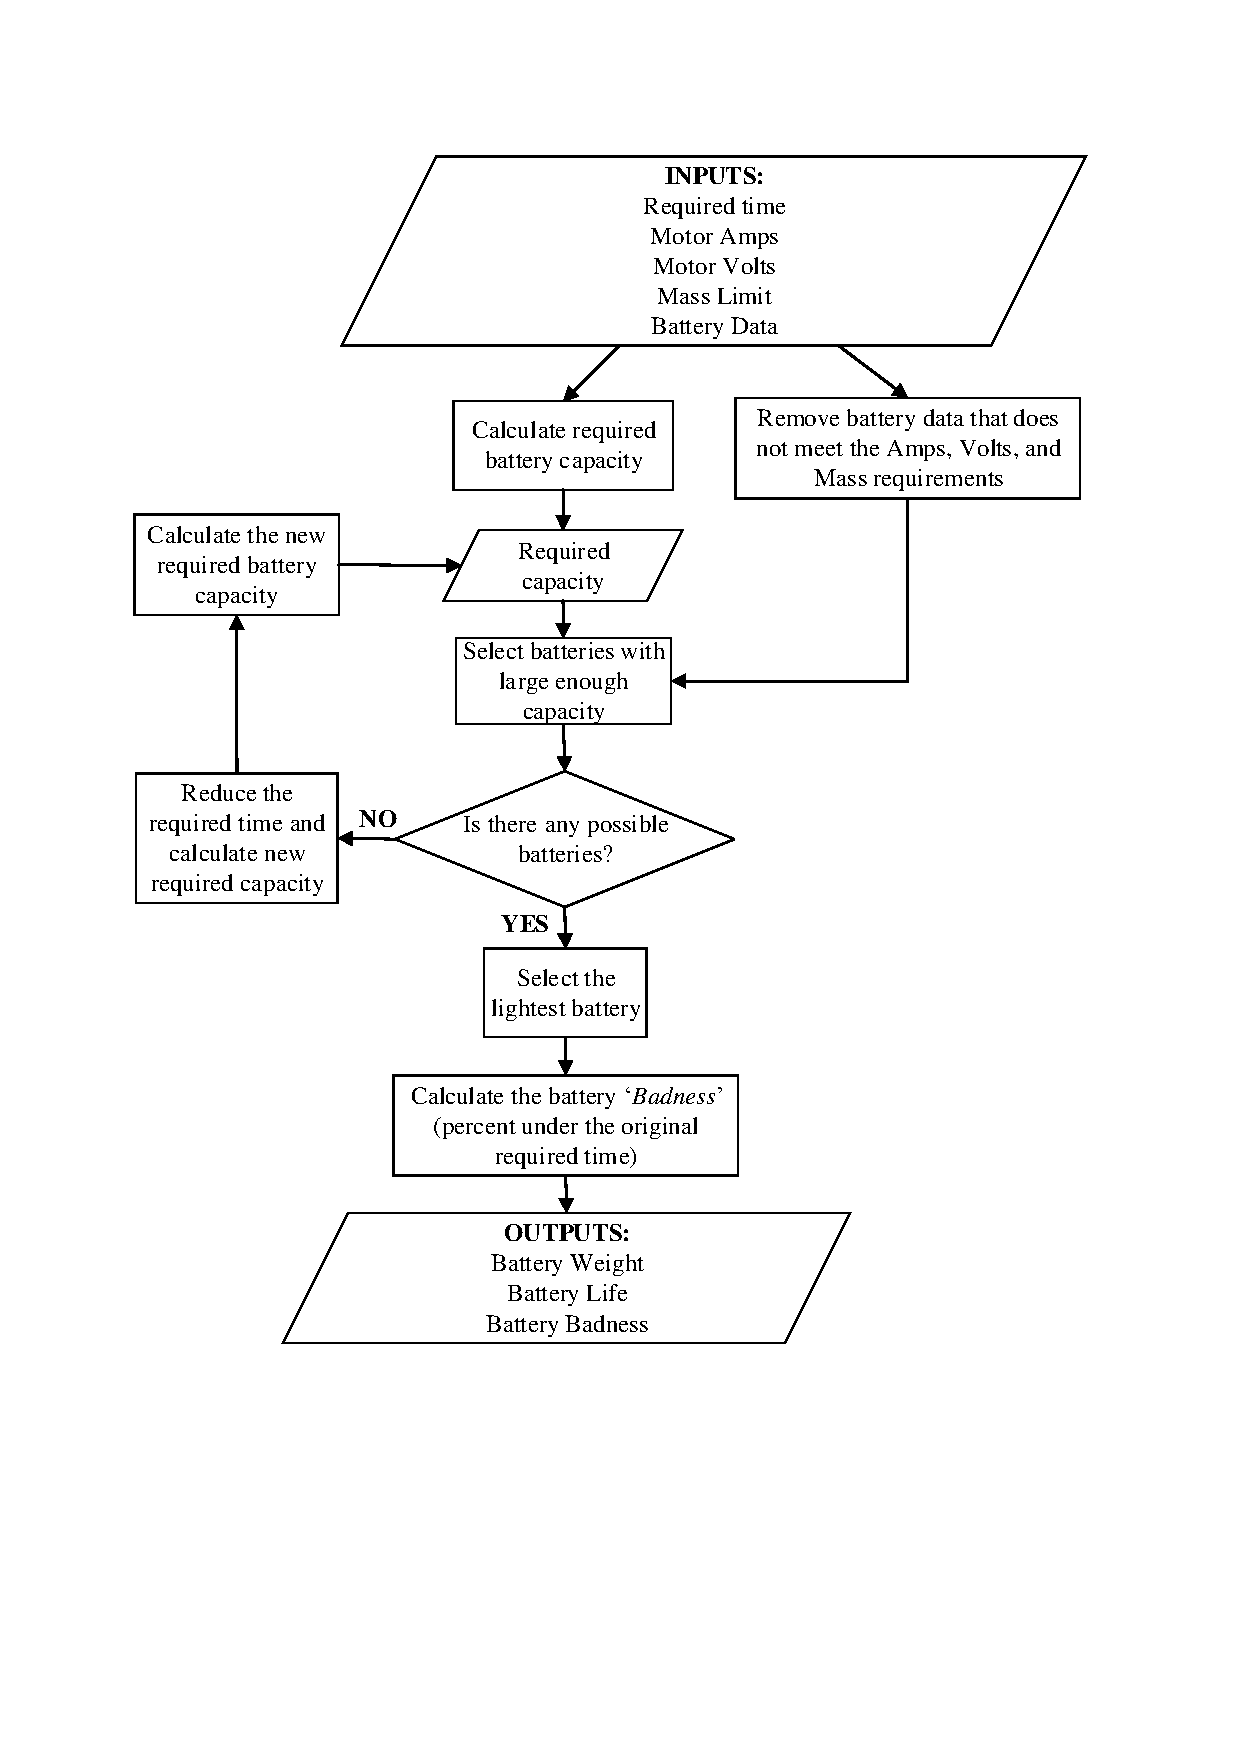
\includegraphics[width=0.95\linewidth]{img/paramaterization/batteryChoice.pdf}
	\caption{Parametrization Outline For Battery Selection}
	\label{fig:batteryOutline}
\end{figure}


The thruster assembly component selection is the logic that decides what propeller, motor, and a battery is used to power the blimp. This selection is what satisfies the three main parameters given to the program from the GUI. The three parameters are the required carrying capacity, required speed, and required flight time. Additional to this is the envelope dimensions which affect the carrying capacity and the required speed (drag). Since the three main parameters are all related, a dominant parameter is also given through the GUI. This dominant parameter will force the program to meet this value and reduce the other two as necessary.

The thruster assembly selection encompasses most of the program. This is because the selection relies on how much carrying capacity there is for the airship. Regardless of the dominant parameter given there is a minimum required carrying capacity of 200g. The weight of the airship is determined by the fixed weight and the changing weight of the optimized parts. The optimized parts are calculated using the weight and force of the thruster assembly selection. To do this a propeller, motor, and a battery is chosen using all three input parameters. Using the values from these the analysis is done on the blimp. The values resulting from the analysis are then used to decide if the chosen parts will work for the input parameters. If the choice fails to meet the minimum weight criteria or the dominant parameter the program is looped, passing limits on the choices. The limits passed back motor, propeller, and battery selection are set differently for each dominant parameter and will be talked about in different sections. The general form described above is kept roughly constant through the three different programs.

\end{document}